% ==================================================
% CHAPTER 3: Using cosmic muon data for alignment studies
% ==================================================

\chapter{Using cosmic muon data for alignment studies}

The cosmic muon data collected is high in statistics, and the clean trail of ionization left by the muons leaves a clean signal.

% --------------------------------------------------
\section{Measuring alignment using cosmics data}
% --------------------------------------------------

Misalignments can be modeled as passive transformations. Ideally, a misalignment model would be chosen and the parameters (for example, a global offset and rotation for each layer) calculated. To understand the potential of cosmic muon data, it is useful to define a local offset. For each area of a strip layer, the local offset is the offset of the strip pattern in that area with respect to the nominal geometry.  Local offsets systematically change the strip that is hit by a muon passing through the area. The \package{tgc\_analysis/CosmicsAnalysis} software assumes the nominal geometry, so the recorded muon y-position ($y_{cluster}$) is shifted opposite to the local offset ($d_{local}$),
% Maybe useful sentence?: The local offset is a result of the non-conformities in the strip pattern etching and inter-layer misalignments.
\begin{equation}
    y_{cluster} = y_{nom} - d_{local}
    \label{eqn:local_translation}
\end{equation}
% Maybe useful sentence?: The true position of individual cosmic muons is not known, and in the analysis the four detector planes float with respect to a software-implemented origin that is not associated with a fixed physical location.
where $y_{nom}$ is the position of the muon that would have been recorded if there was no local offset. Equation~\ref{eqn:local_translation} ignores other factors that could affect the cluster position (like resolution). The local offset is unknown and there is no external reference to measure $y_{nom}$. Therefore, only relative alignment parameters can be extracted. The minimal relative coordinate system uses two reference or fixed layers~\cite{lefebvre_thesis}. The hits on the two fixed layers are used to create a track that can be interpolated or extrapolated to the other two layers. The residual of track $i$, $\Delta_i$ is defined as,
\begin{equation}
    \Delta_i = y_{i,hit} - y_{i,track}
    \label{eqn:residual}
\end{equation}

Track residuals are affected by the local offset in the area of each layer's hit. As an example, in figure~\ref{fig:fake_event_display}, layers 1 and 4 are used as reference, and the residual on layer 2 perhaps indicates that in the area of the track, layer 3 is offset with respect to layers 1 and 4. However, there is no way to parse out if is it really layer 2 that is offset with respect to the nominal geometry, or some combination of offset on all three layers that causes the residual.

\begin{figure}
    \centering
    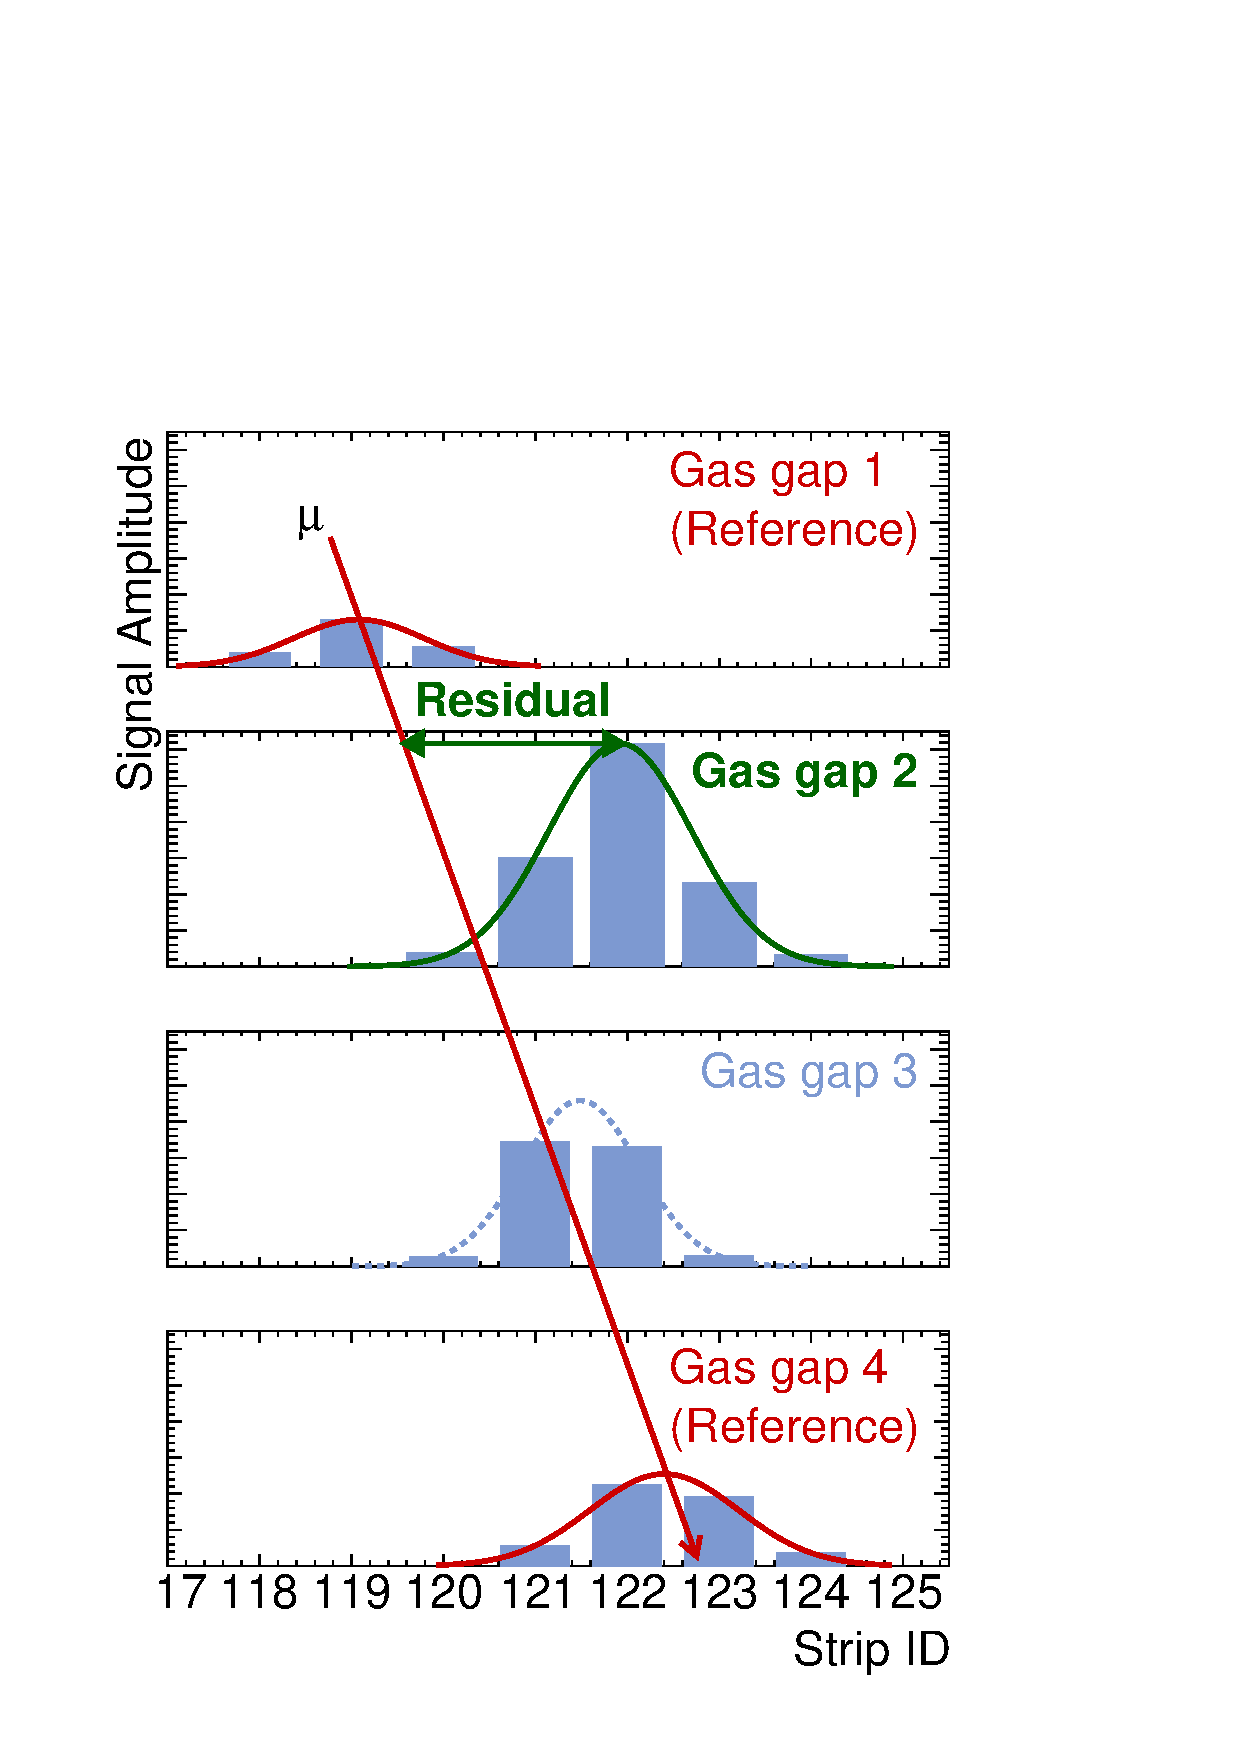
\includegraphics[width = 0.95\textwidth]{figures/figure_fake_event_display.pdf}
    \caption{Representation of a muon event recorded by an sTGC. The clusters are fit with a Gaussian and the mean is taken as the hit position. A track is built from the chosen reference layers, 1 and 4, and the residual calculated on layer 2.}
    \label{fig:fake_event_display}
\end{figure}

Of course, a single track residual says nothing of the real relative local offset thanks to the limited spatial resolution of the detectors and tracks caused by noise or delta rays contributing large residuals. However, the mean of residuals for all tracks in a local area will be shifted systematically by the local offsets between layers~\cite{lefebvre_thesis}. 

